\documentclass[16pt]{beamer}
\usepackage[utf8]{inputenc}
\usepackage{media9}
\usepackage{amsmath}
\usepackage{amsfonts}
\usepackage{amssymb}
\usepackage{amsthm}
\usepackage{graphicx,epsfig}
\usepackage{xcolor}
 
\usetheme{Madrid}
\usecolortheme{beaver}

\usepackage{anyfontsize}

\setbeamertemplate{itemize/enumerate body begin}{\large}
\setbeamertemplate{itemize/enumerate subbody begin}{\large}

%gets rid of bottom navigation bars
\setbeamertemplate{footline}[frame number]{}

%gets rid of bottom navigation symbols
\setbeamertemplate{navigation symbols}{}

%gets rid of footer
%will override 'frame number' instruction above
%comment out to revert to previous/default definitions
\setbeamertemplate{footline}{}
 
%Information to be included in the title page:
\title[Instability Bubbles]{Periodic Multi-Pulses in Hamiltonian Systems with Symmetry}
\titlegraphic{\includegraphics[width=0.3\textwidth]{images/babyelephant1.jpg}}

\author[Parker, R.] % (optional, for multiple authors)
{Ross Parker\inst{1} \and Bj\"{o}rn Sandstede\inst{2}}

\institute[SMU] % (optional)
{
  \inst{1}
  Southern Methodist University
  \and
  \inst{2}
  Brown University
}

\date[23 May, 2021]
{SIAM Conference on Applications of Dynamical Systems 2021 \\ 23 May, 2021}

\AtBeginSection[]
{
  \begin{frame}
    \frametitle{Outline}
    \tableofcontents[currentsection]
  \end{frame}
}
 
\begin{document}
 
\frame{\titlepage}
 
\begin{frame}
\frametitle{Outline}
\tableofcontents
\end{frame}

\section{Background and Motivation}

\begin{frame}
	\frametitle{Hamiltonian PDEs with symmetry}   
	\begin{center}
	\Large
		\[ u_t = \partial_x \mathcal{E}'(u) \]
	\end{center}

	\begin{itemize}
		\item $\mathcal{E}(u)$ is conserved energy
		\vspace{0.5cm}
		\item Symmetries:
		\begin{itemize}
			\item Reversibility
			\item Translation invariance
		\end{itemize}
	\end{itemize}
\end{frame}

\begin{frame}
	\frametitle{Fifth-order KdV equation (KdV5)}   
	\begin{center}
	\Large
		\[ u_t = u_{xxxxx} - u_{xxx} - 2 u u_x  \]
	\end{center}

	\begin{itemize}
		\item Weakly nonlinear long wave approximation to capillary-gravity wave problem
		\item Wavelength long compared to wave depth
		\item Influenced by surface tension and gravity
		\item Additional applications to nonlinear optics and plasma physics
	\end{itemize}
\end{frame}


\begin{frame}
	\frametitle{Traveling waves}
	\begin{itemize}
		\item In co-moving frame with speed $c$
		\begin{align*} 
		u_t = u_{xxxxx} - u_{xxx} + c u_x - 2 u u_x
		\end{align*}

		\item Hamiltonian formulation
		\begin{align*} 
			u_t &= \partial_x \mathcal{E}'(u) \\
			\mathcal{E}(u) &= -\int_{-\infty}^{\infty} \left( \frac{1}{2}u_{xx}^2 + \frac{1}{2}u_x^2 + \frac{1}{2}cu^2 - \frac{1}{3}u^3 \right) dx 
		\end{align*}

		\item Reversible and translation invariant

		\item Localized equilibrium solutions satisfy 4th order ODE: $\mathcal{E}'(u) = 0$
		\begin{align*} 
		u_{xxxx} - u_{xx} + cu - u^2 = 0
		\end{align*}
	\end{itemize}
\end{frame}


\begin{frame}
	\frametitle{Spatial dynamics perspective}
	\begin{itemize}
		\item Write as dynamical system in $\mathbb{R}^4$ evolving in spatial variable $x$
		\begin{align*}
		\frac{d}{dx}\begin{pmatrix}u_1 \\ u_2 \\ u_3 \\ u_4 \\ \end{pmatrix} =
		\begin{pmatrix}u_2 \\ u_3 \\ u_4 \\ u_3 - c u_1 + u_1^2  \\ \end{pmatrix}
		\end{align*}
		\item Saddle point equilibrium at 0
		\begin{center}
		\includegraphics[width=0.7\textwidth]{images/eigbifurcation2}
		\end{center}
		For $c > 1/4$, quartet $\pm \alpha \pm \beta i$
	\end{itemize}
\end{frame}


\begin{frame}
	\frametitle{Homoclinic orbits}

	\begin{itemize}
		\item Localized pulse solutions are homoclinic orbits
		\item For KdV5, symmetric homoclinic orbits exist for $c > 0$\footnote{Groves (1998), Chugunova and Pelinovsky (2007)}
		\item Oscillatory tails for $c > 1/4$
	\end{itemize}

	\begin{figure}
   		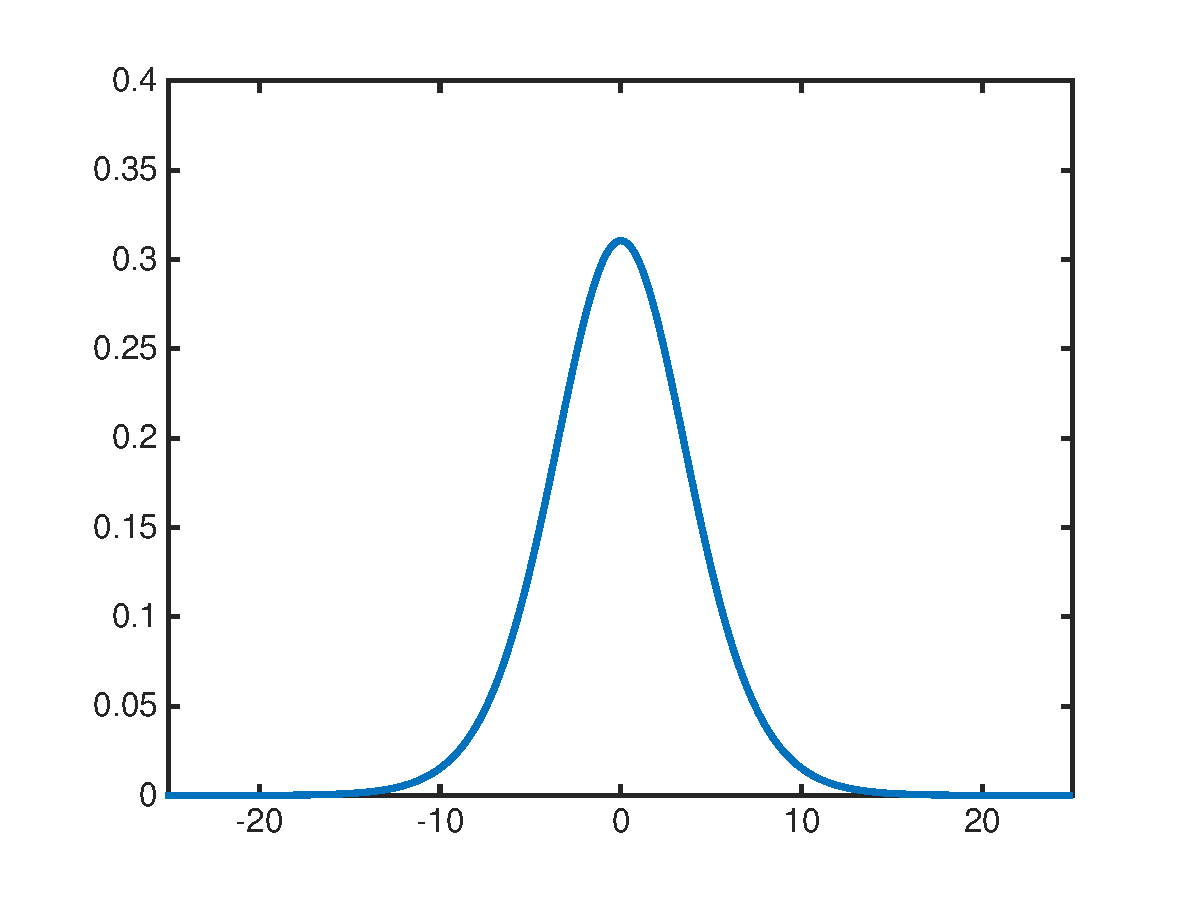
\includegraphics[width=0.48\textwidth]{images/exactsol}
   		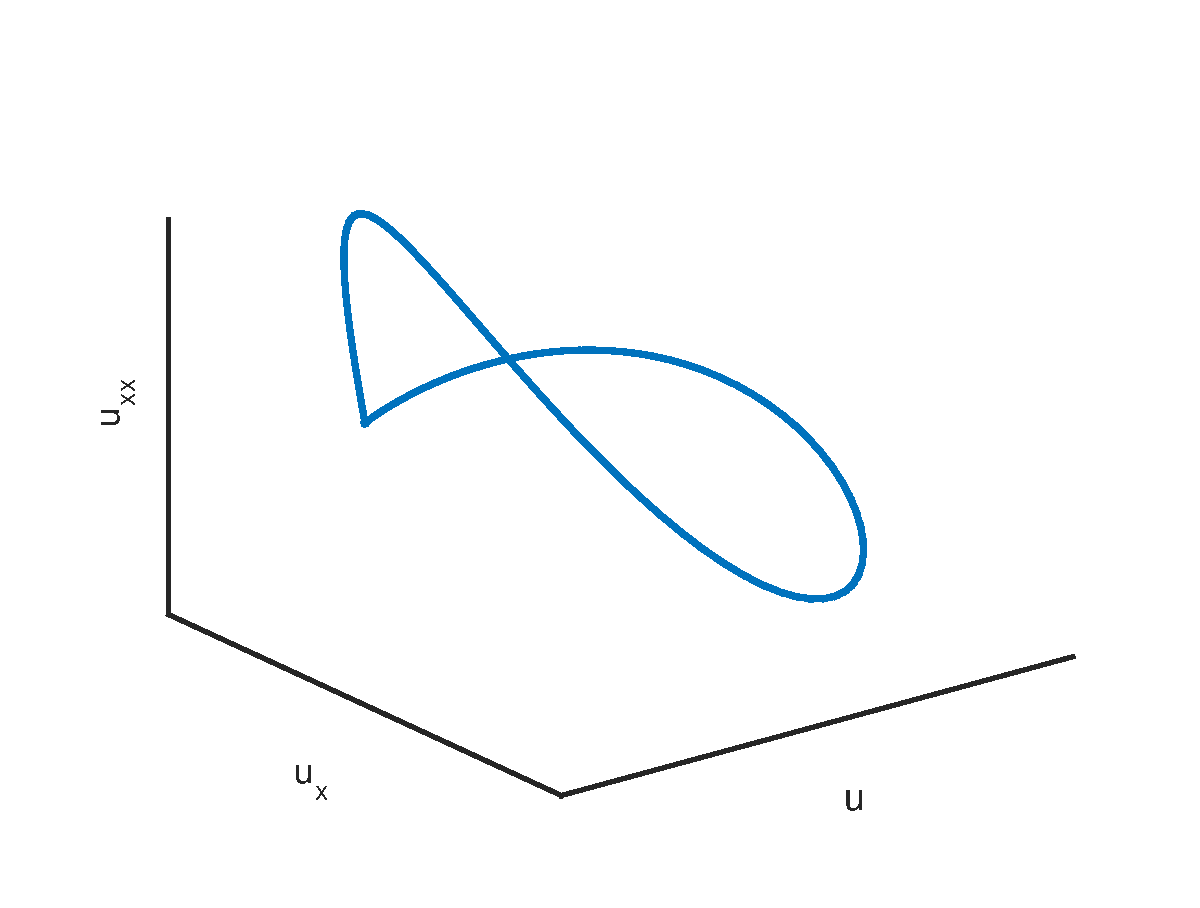
\includegraphics[width=0.48\textwidth]{images/exactsolorbit}
	\end{figure}
\end{frame}

\begin{frame}
\frametitle{Multi-pulses} 
    \begin{block}{Theorem [Buffoni et al. (1996); Sandstede (1997)]}
    \large
    For $c > 1/4$, multi-pulse solutions exist.
    \begin{itemize}
    	\item Multi-loop homoclinic orbits
    	\item Constructed by gluing single pulses end-to-end
    \end{itemize}

	\begin{figure}
	\begin{center}
	\includegraphics[width=7.5cm]{images/multipulse.png}
	\end{center}
	\begin{align*}
	 X_j &\approx \frac{2 \pi}{\beta} k_j + C && k_j \text{ integer}
	\end{align*}
	\end{figure}

    \end{block}
\end{frame}

\begin{frame}
	\frametitle{Double pulse construction}
	\begin{figure}
	\begin{center}
	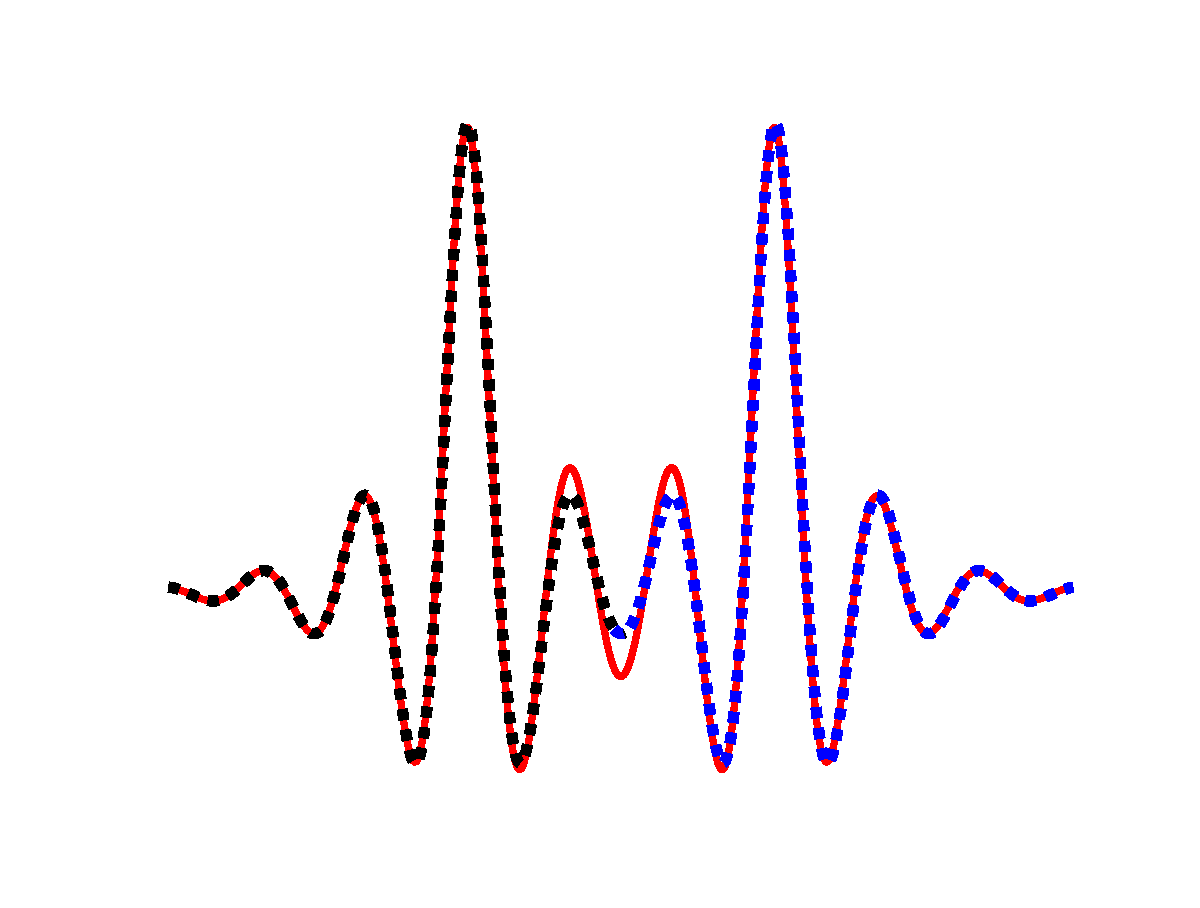
\includegraphics[width=0.7\linewidth]{images/dpconstruction.eps}
	\end{center}
	\end{figure}
	Tail oscillations of neighboring pulses have to ``match up''.
\end{frame}


\begin{frame}
	\frametitle{Double pulse solutions}
	\begin{figure}
	\begin{center}
	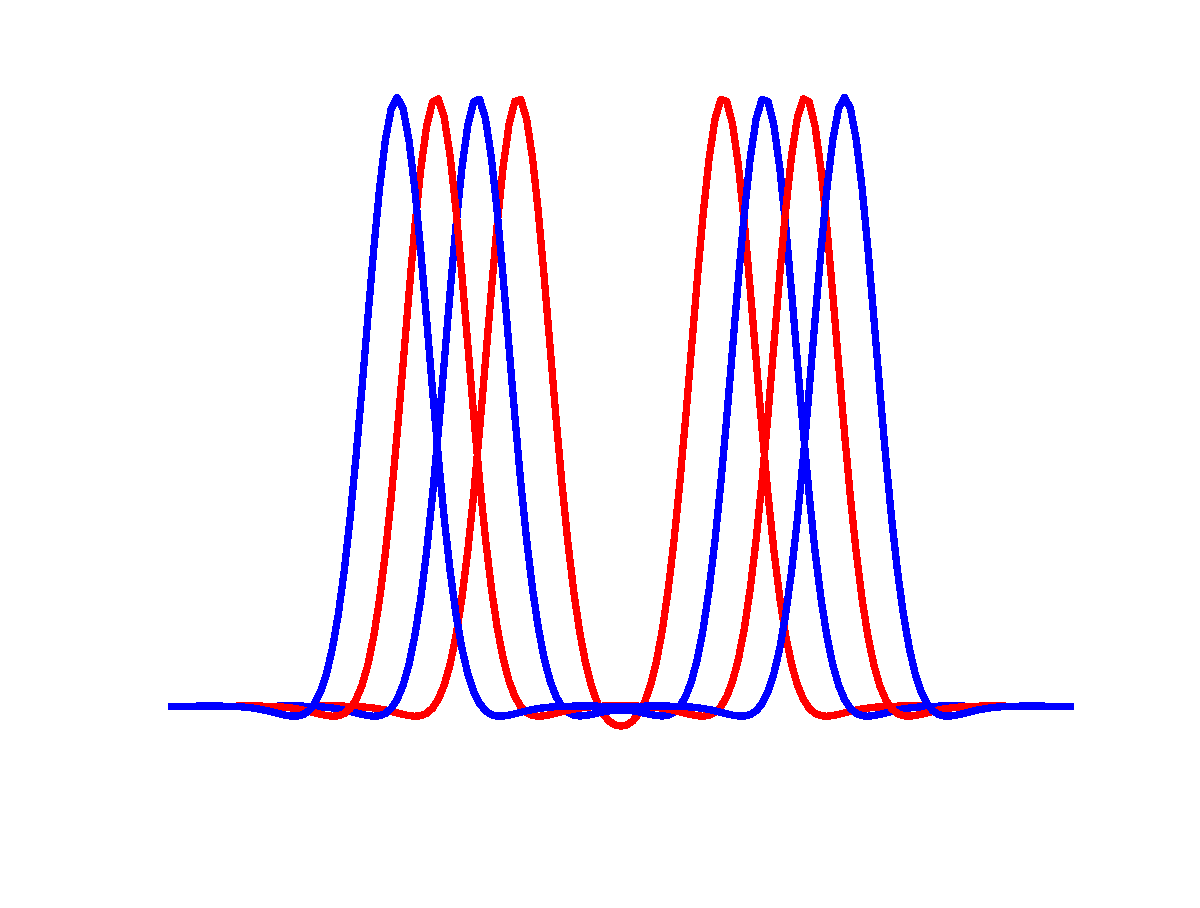
\includegraphics[width=0.7\linewidth]{images/first4dp}
	\end{center}
	\end{figure}
	Construction of first four double pulses ($c = 10$). \textcolor{red}{$k$ odd}. \textcolor{blue}{$k$ even}.
\end{frame}

\section{Spectrum of multi-pulses}

\begin{frame}
	\frametitle{Are multi-pulses stable?}
	\begin{itemize}
	\item What happens when we perturb a multi-pulse?
	\vspace{0.25cm}
	\item First step: spectrum of linearization about multi-pulse
	\begin{itemize}
		\item Nonlinear interactions between neighboring pulses captured by eigenvalues near 0
		\vspace{0.25cm}
		\item These \textbf{interaction eigenvalues} suggest what happens when a multi-pulse is perturbed
		\vspace{0.25cm}
		\item Eigenvalues must come in quartets since Hamiltonian system
			\begin{center}
				\includegraphics[width=0.6\linewidth]{images/eigdouble2}
			\end{center}
		\vspace{0.25cm}
		\item Best we can hope for is ``neutral stability''
	\end{itemize}
	\end{itemize}
\end{frame}

\begin{frame}
	\frametitle{Eigenvalue problem}
	Linearization of the PDE about an equilibrium solution $u^*(x)$

	\begin{center}
		$(\mathcal{L} - \lambda I )v = 0$
	\end{center}

	\begin{center}
		$\mathcal{L} = \partial_x^5 - \partial_x^3 + (c - 2 u^*)\partial_x - 2 u^*_x $
	\end{center}

	\begin{itemize}
		\item Resolvent set: $\mathcal{L} - \lambda I$ is invertible with bounded inverse
		\vspace{0.5cm}
		\item Spectrum: complement of resolvent set
		\begin{itemize}
		\item Essential spectrum: $\mathcal{L} - \lambda I$ is not Fredholm
		\vspace{0.25cm}
		\item Point spectrum (eigenvalues): kernel of $\mathcal{L} - \lambda I$ contains an 	eigenfunction which lies in the underlying space.
		\end{itemize}
	\end{itemize}
\end{frame}


\begin{frame}
	\frametitle{Essential spectrum}
	\begin{itemize}
		\item Essential spectrum is entire imaginary axis
		\vspace{0.5cm}
			\begin{center}
			\includegraphics[width=0.3\linewidth]{images/essspec1.eps}
			\end{center}
		\vspace{0.5cm}
		\item Depends only on background state.
	\end{itemize}
\end{frame}


\begin{frame}
	\frametitle{Point spectrum}
	\begin{itemize}
		\item Always have eigenvalue at 0 with algebraic multiplicity 2 from translation invariance
		\vspace{0.5cm}
		\begin{center}
			\includegraphics[width=0.3\linewidth]{images/eigsingle.eps}
		\end{center}
		\vspace{0.5cm}
		\item Eigenfunctions are $\partial_x u^*(x)$ and $\partial_c u^*(x)$
	\end{itemize}
\end{frame}

\begin{frame}
	\frametitle{Spectrum of multi-pulses}
	\begin{itemize}
	\item Spectrum of primary pulse
		\begin{center}
			\includegraphics[width=0.2\linewidth]{images/eigsinglepulse.eps}
		\end{center}
	\item Multi-pulses: additional eigenvalues near 0 from interaction between neighboring pulses\footnote{Sandstede (1998)}
 	\item Interaction eigenvalues must come in quartets
		\begin{center}
			\includegraphics[width=0.8\linewidth]{images/eigdouble2}
		\end{center}
	\end{itemize}
\end{frame}

\begin{frame}
	\frametitle{Spectrum of double pulses}
	\begin{center}
		\includegraphics[width=0.8\linewidth]{images/dpsplit}
	\end{center}
\end{frame}

\begin{frame}
	\frametitle{Unstable double pulses ($k$ odd)}
	\begin{center}
		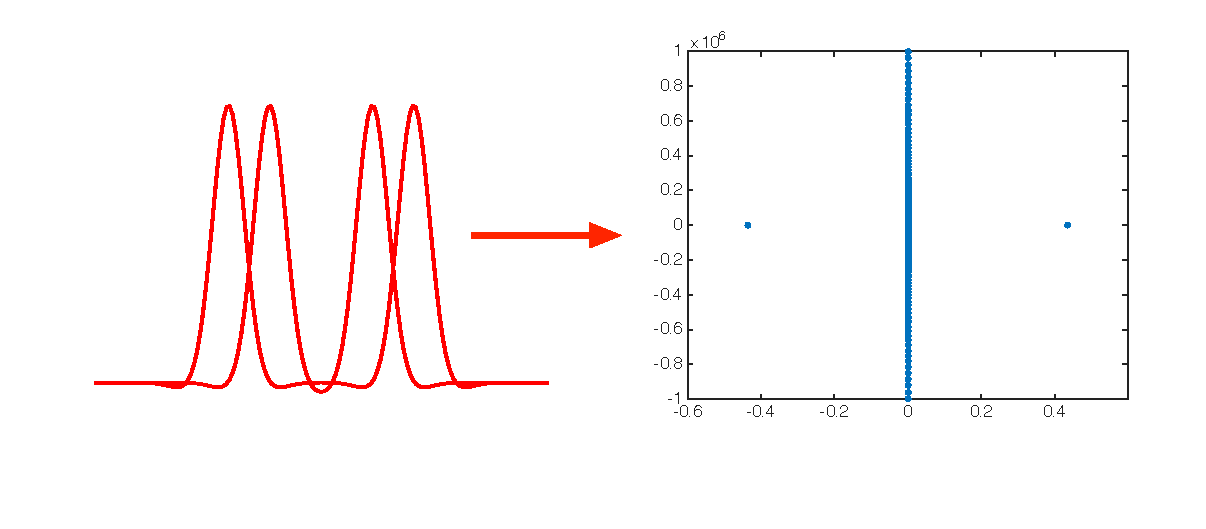
\includegraphics[width=1\linewidth]{images/doubleunstableeig}
	\end{center}
	\begin{itemize}
	\item Pair of real interaction eigenvalues.
	\end{itemize}
\end{frame}

\begin{frame}
	\frametitle{Neutrally stable double pulses ($k$ even)}
	\begin{center}
		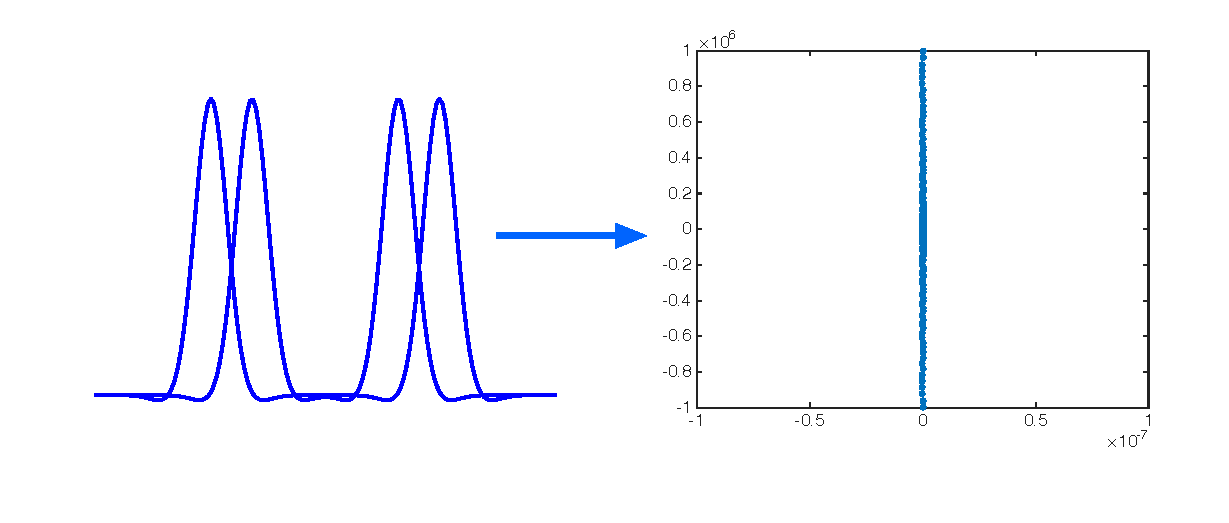
\includegraphics[width=1\linewidth]{images/doublestableeig}
	\end{center}
	\begin{itemize}
	\item Where are the interaction eigenvalues?
	\item Embedded in the essential spectrum?
	\item How would you locate them?
	\end{itemize}
\end{frame}

\section{Multi-pulses on a periodic domain}

\begin{frame}
	\frametitle{Multi-pulses on a periodic domain}

	\begin{itemize}
		\item Essential spectrum becomes discrete
		\vspace{0.5cm}
		\item Don't have to look for embedded eigenvalues
		\vspace{0.5cm}
		\item Restricted to investigating stability with respect to co-periodic perturbations
	\end{itemize}
\end{frame}

\begin{frame}
	\frametitle{Additional symmetry on periodic domain}

	\begin{itemize}
		\item Equilibrium solutions can satisfy
		\begin{align*}
		\mathcal{E}'(u) &= k && k \in \mathbb{R}
		\end{align*}
		\item For nonzero $k$, solutions decay to nonzero baseline.
		\begin{center}
			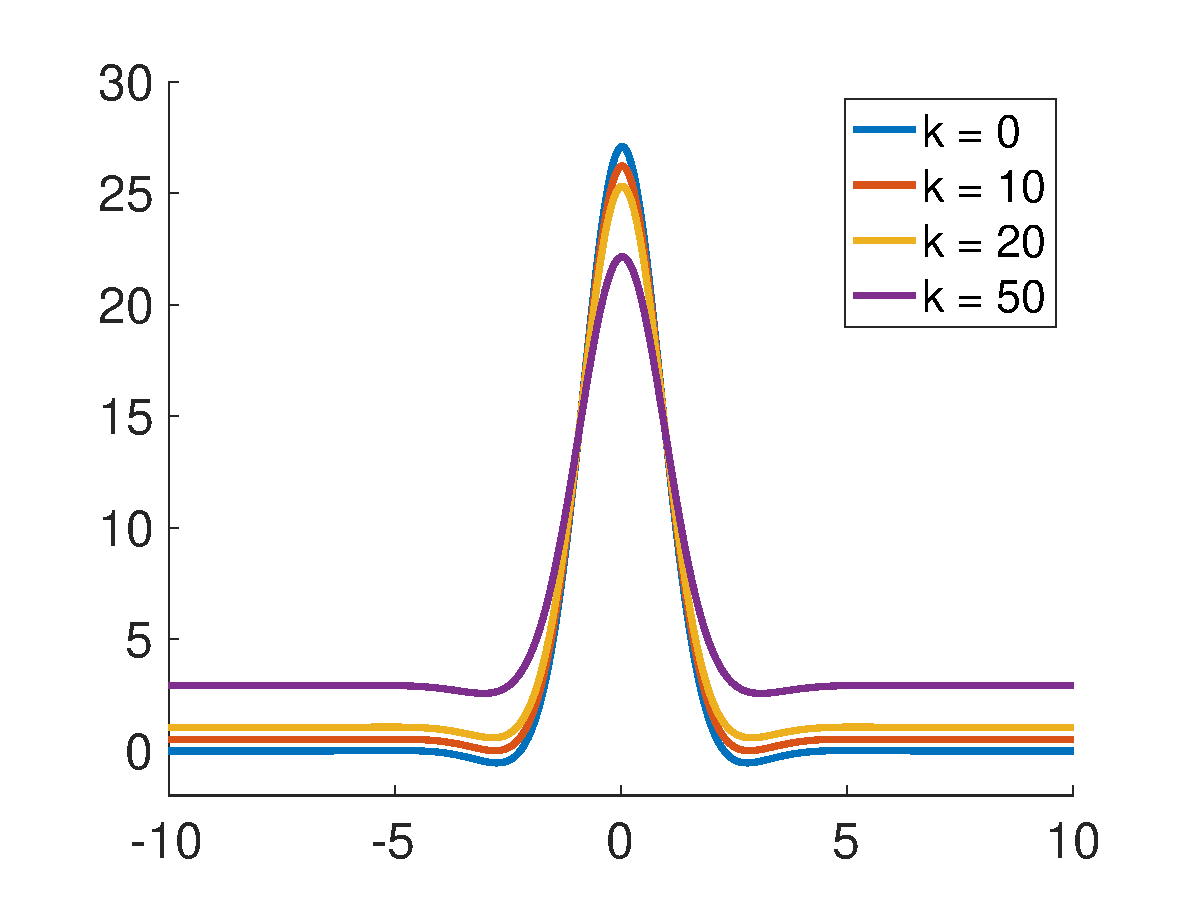
\includegraphics[width=0.5\linewidth]{images/periodick.eps}
		\end{center}
		\item Additional kernel eigenfunction: $\partial_k u^*(x)$
	\end{itemize}
\end{frame}

\begin{frame}
\frametitle{Periodic multi-pulses} 
    \begin{block}{Theorem [P.]}
    For sufficiently large $X_j$, periodic multipulse solutions exist.\footnote{Some restrictions apply.}
    \begin{itemize}
    	\item Multi-loop periodic orbits
		\item Constructed by gluing single pulses end-to-end in a loop
		\item One more length parameter for periodic multi-pulse
    \end{itemize}

	\begin{figure}
	\begin{center}
	\includegraphics[width=7cm]{images/multipulseperiodic.png}
	\end{center}
	\end{figure}
    \end{block}
\end{frame}

\begin{frame}
\frametitle{Periodic double pulses} 
    \begin{block}{Theorem [P.]}
    Asymmetric 2-periodic pulses ($X_0 \neq X_1$) bifurcate from symmetric 2-periodic pulses ($X_0 = X_1$) in a series of pitchfork bifurcations.

	\begin{figure}
	\begin{center}
	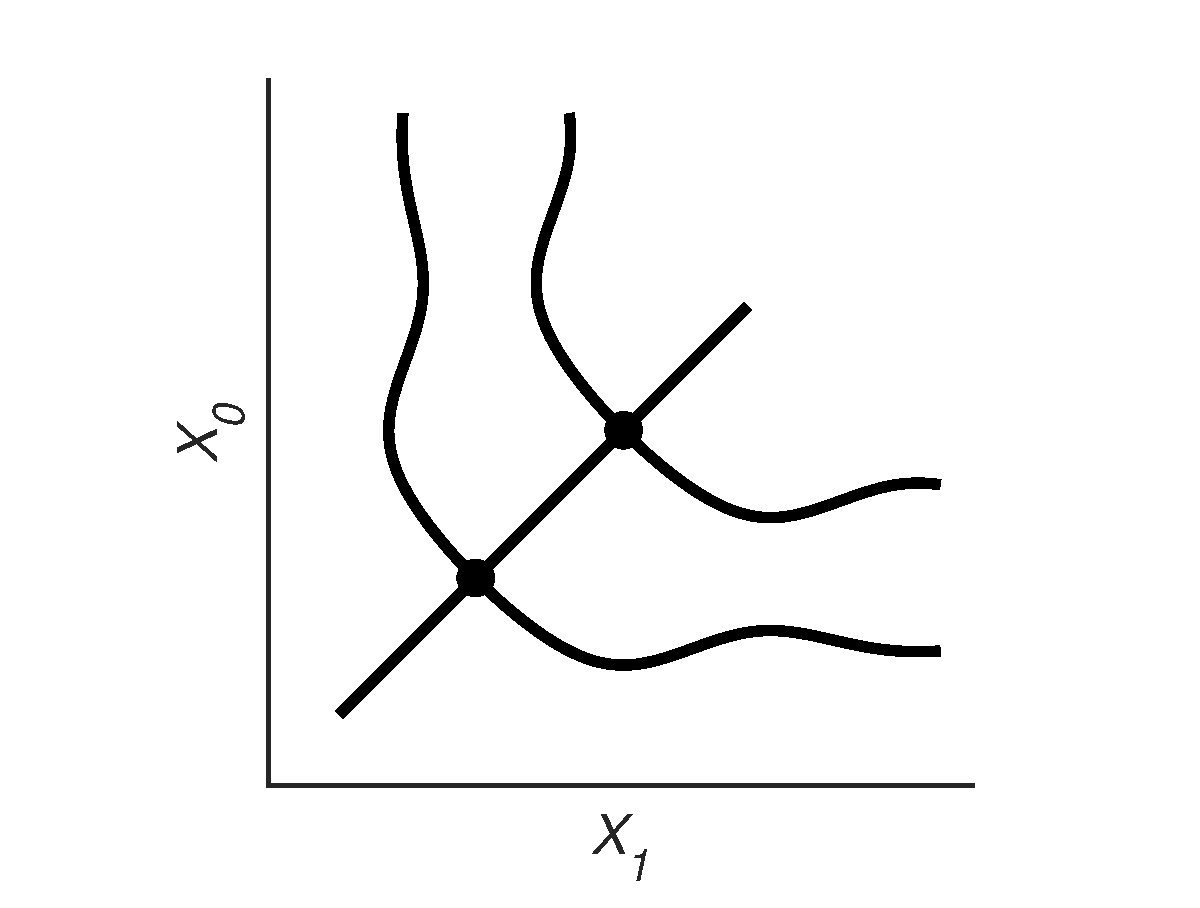
\includegraphics[width=7.25cm]{images/periodicpitchfork.eps}
	\end{center}
	\end{figure}
    \end{block}
\end{frame}

\begin{frame}
	\frametitle{Three Groups of Eigenvalues}
	\large

	\begin{itemize}
		\item Kernel eigenvalues 
		\begin{center}
			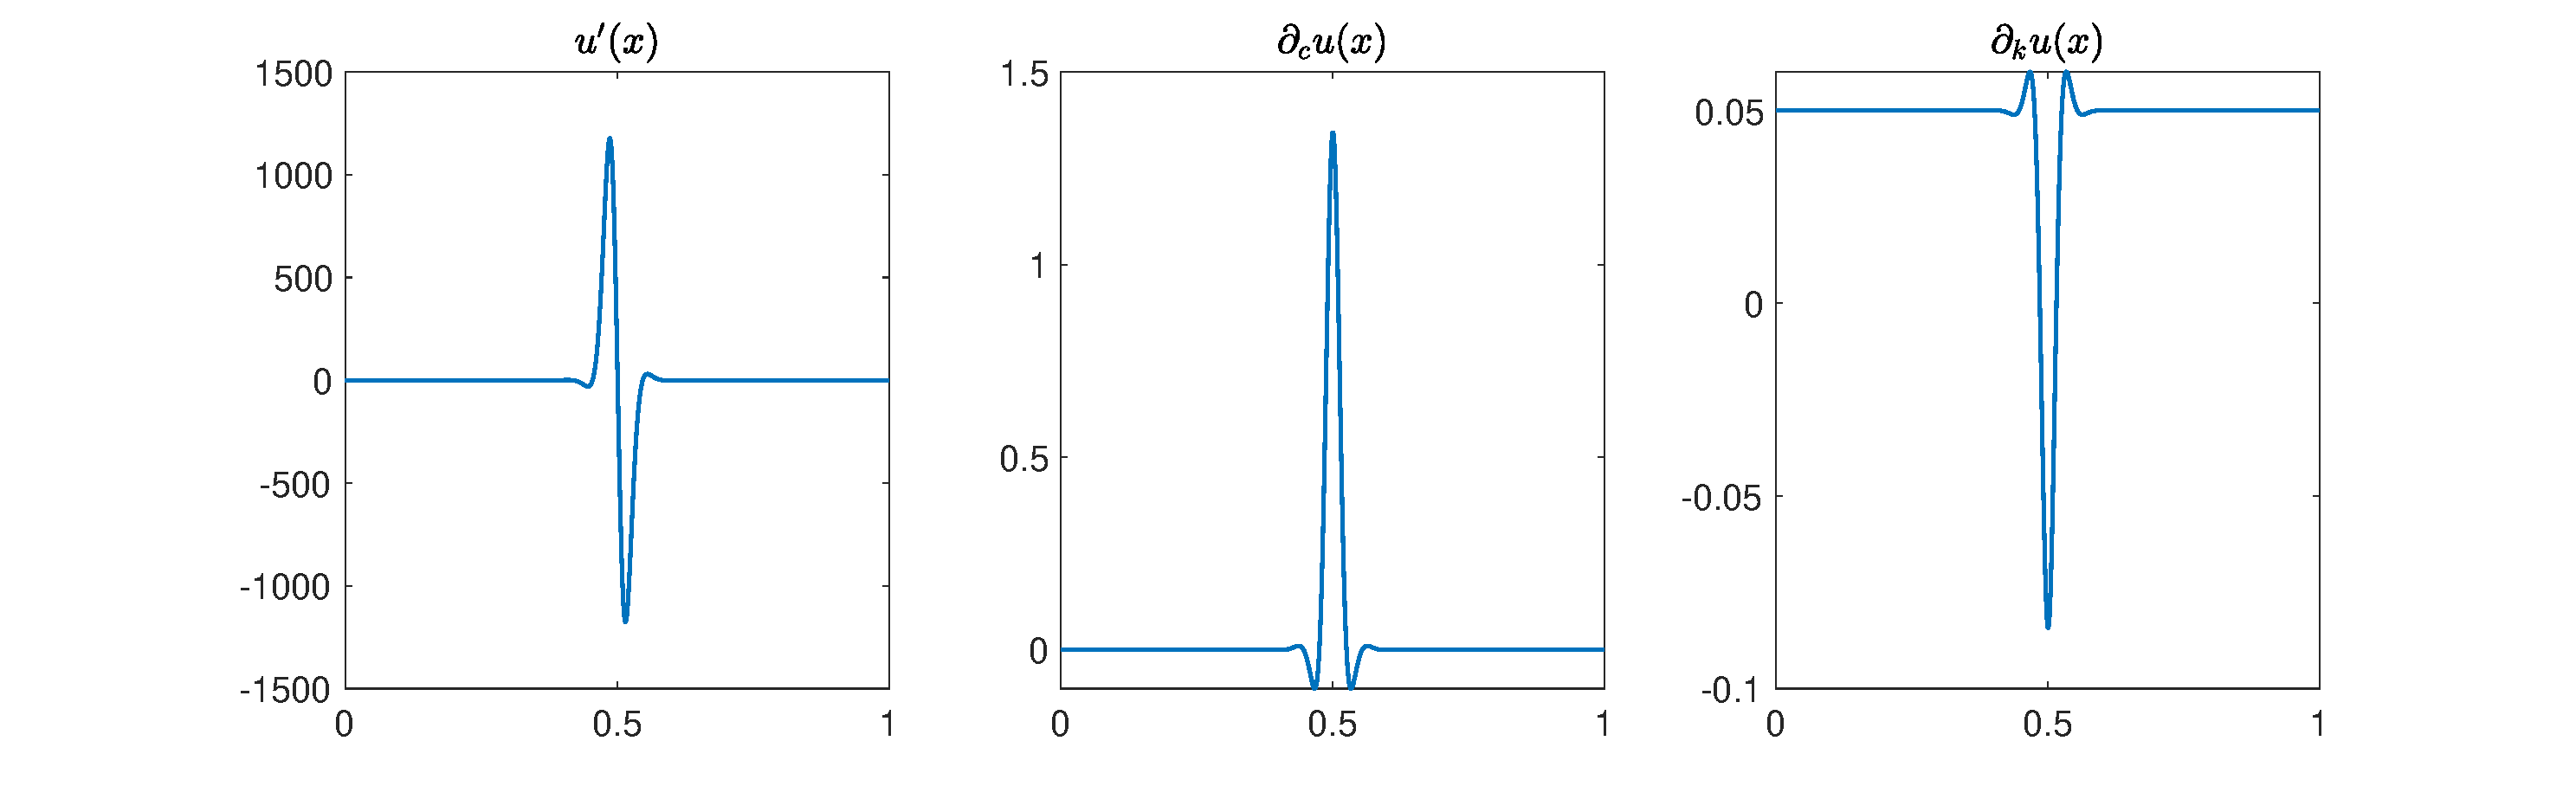
\includegraphics[width=12cm]{images/perkernel.eps}
			\end{center}
		\item ``Essential spectrum'' eigenvalues
		\begin{itemize}
			\item On imaginary axis
			\item Depend (to leading order) only on background state and domain size (period)
		\end{itemize}
		\item Interaction eigenvalues
		\begin{itemize}
			\item Each pulse interacts with two neighbors
			\item Depend on geometry of periodic multi-pulse
		\end{itemize}
	\end{itemize}
	\vspace{0.5cm}
\end{frame}

\begin{frame}
\frametitle{Construction of eigenfunctions}
\begin{itemize}
\item Heuristic: for double pulse 
	\[ u_2(x) = u(x+L) + u(x-L) + \text{``h.o.t.''} \]
    	\begin{figure}
		\begin{center}
		% 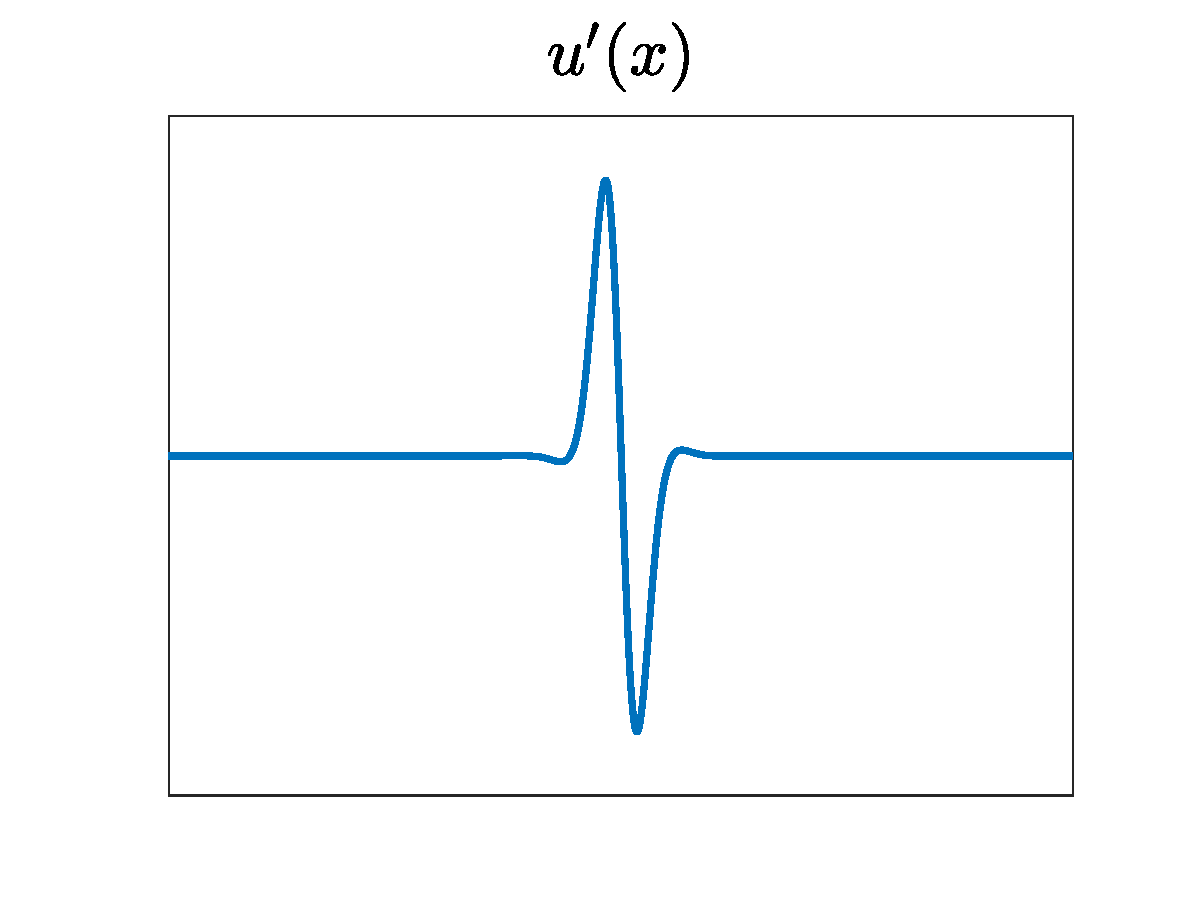
\includegraphics[width=4cm]{images/singleprime.eps}
		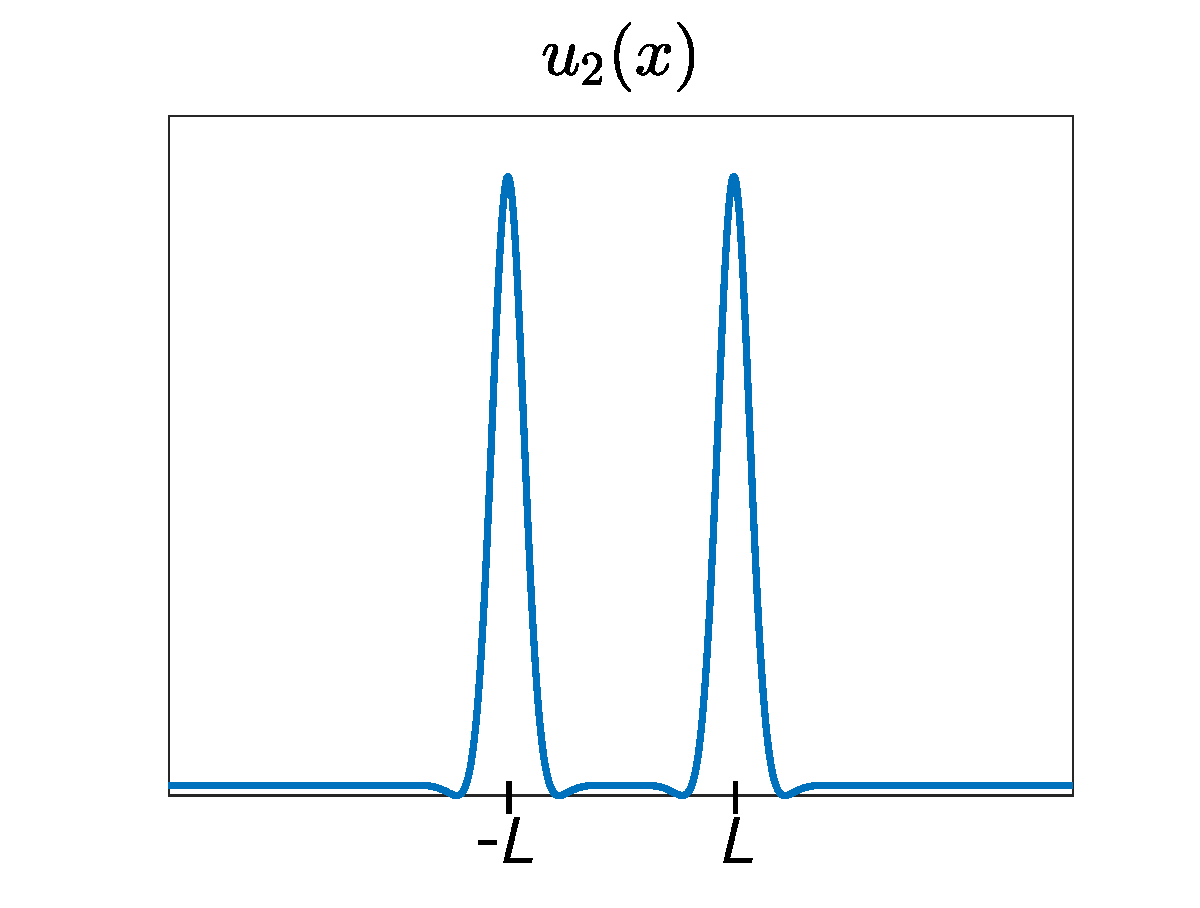
\includegraphics[width=4cm]{images/doubleplain.eps}
		\end{center}
		\end{figure}
	use linear combination ansatz for eigenfunction
\begin{align*}
v(x) = d_0 u'(x+L) + d_1 u'(x-L) + w(x)
\end{align*}
\item $w(x)$ is a small remainder term
\item Solve for constants $d_0$ and $d_1$ (and remainder term)
\end{itemize}
\end{frame}

\begin{frame}
\frametitle{Construction of eigenfunctions}
\begin{itemize}
\item Eigenfunction $v(x)$ is linear combination of translates of $u'(x)$ to leading order.
    	\begin{figure}
		\begin{center}
		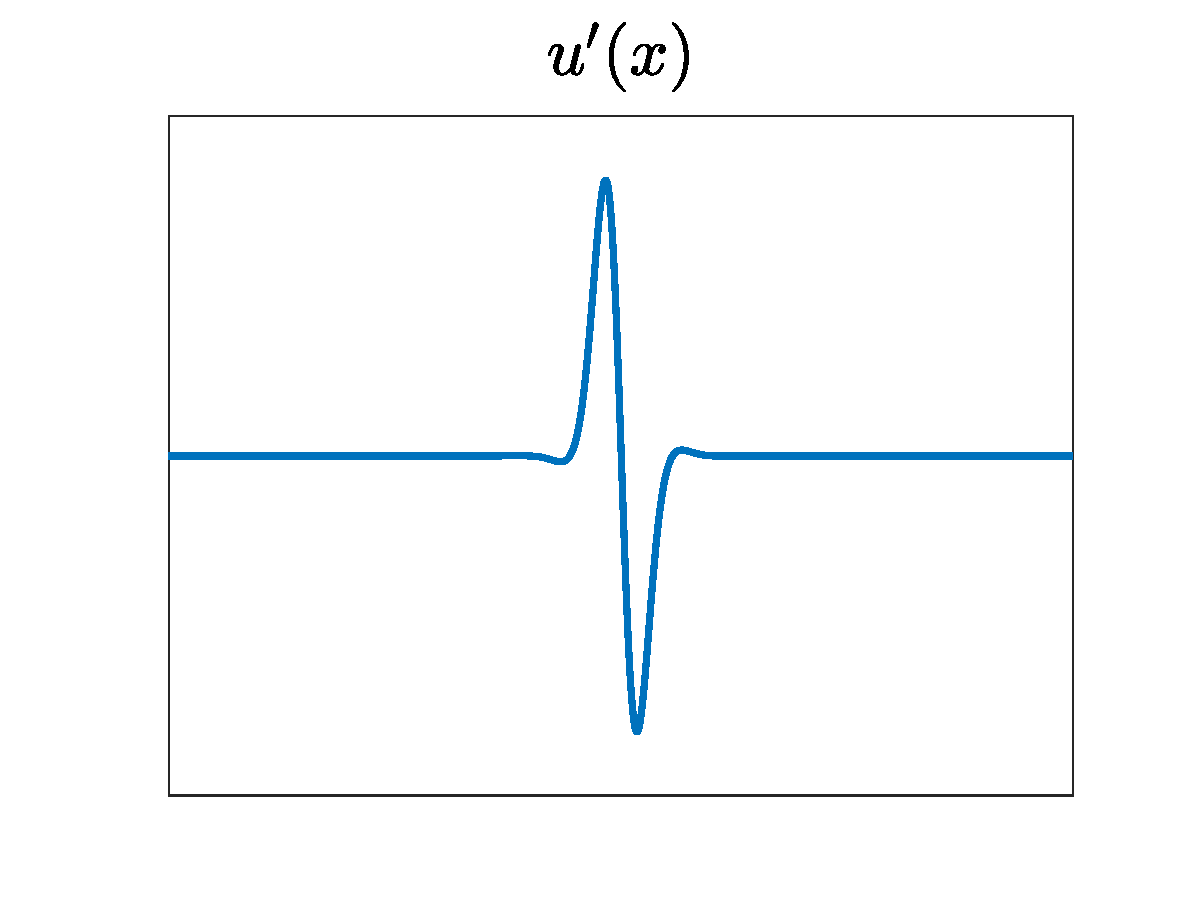
\includegraphics[width=5cm]{images/singleprime.eps}
		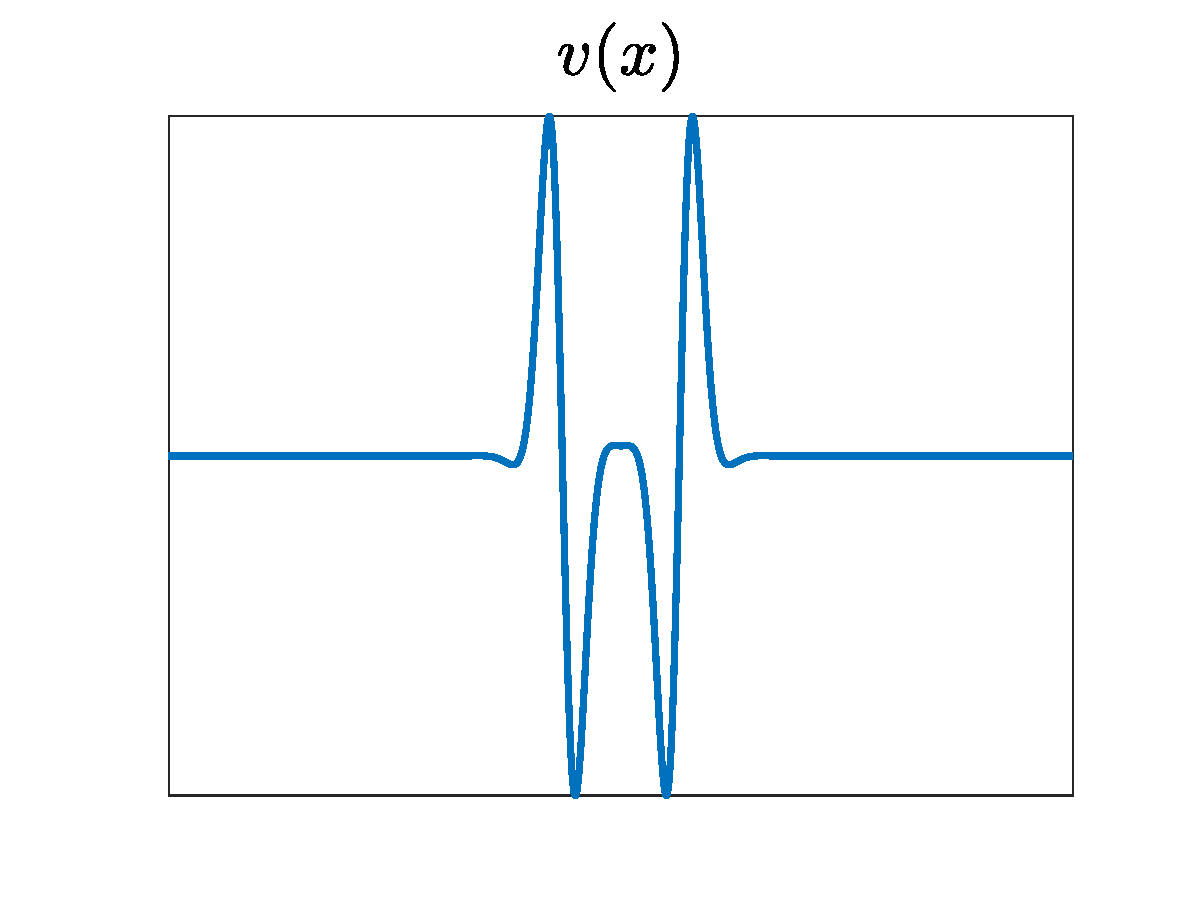
\includegraphics[width=5cm]{images/eigenfunction.eps}
		\end{center}
		\end{figure}
\item Actual ansatz involves all three kernel eigenfunctions
\begin{itemize}
	\item $u'(x)$
	\item $\partial_c u(x)$
	\item $\partial_k u(x)$
\end{itemize}
\vspace{0.25cm}
\item Solution technique: Lin's method (Lyapunov-Schmidt reduction)
\end{itemize}
\end{frame}

\begin{frame}
\frametitle{Matrix reduction} 
    \begin{block}{Theorem [P.]}
    $\lambda$ is a eigenvalue for the linearization of the PDE about a periodic $n-$pulse on $[-X, X]$ if and only if 
    \[
    \det\left[ \begin{pmatrix}
	K(\lambda) - \frac{1}{2} \lambda \tilde{M} K^+(\lambda) & \lambda^2 M_c I \\
	-\frac{1}{2} \lambda M_c K^+(\lambda) & A - \lambda^2 MI 
	\end{pmatrix} + \text{``h.o.t.''} \right]= 0.
    \]
    \end{block}
    \begin{itemize}
		\item This is essentially an Evans function
    	\item Each block in the block matrix is $n \times n$
    	\item Matrices $K(\lambda)$, $K^+(\lambda)$ only involve length parameters $X_k$
    	\item Matrix $A$ involves tails of primary pulse 
    	\item Constants $M$, $M_c$, and $\tilde{M}$ are Melnikov-type integrals involving primary pulse and its kernel eigenfunctions
    \end{itemize}
\end{frame}

\begin{frame}
\frametitle{Matrix reduction} 
For a periodic 2-pulse, the matrix is 
\[
\begin{pmatrix}
e^{-\frac{\lambda}{c}X_1} -\frac{1}{2}\lambda \tilde{M} e^{-\frac{\lambda}{c}X_1} & -e^{\frac{\lambda}{c}X_0} -\frac{1}{2}\lambda \tilde{M} e^{\frac{\lambda}{c}X_0} & M_c \lambda^2 & 0 \\
-e^{\frac{\lambda}{c}X_1} -\frac{1}{2}\lambda \tilde{M} e^{\frac{\lambda}{c}X_1} & e^{-\frac{\lambda}{c}X_0} -\frac{1}{2}\lambda \tilde{M} e^{-\frac{\lambda}{c}X_0} & 0 & M_c \lambda^2 \\
-\frac{1}{2}\lambda M_c e^{-\frac{\lambda}{c}X_1} & -\frac{1}{2}\lambda M_c e^{\frac{\lambda}{c}X_0} &-a-\lambda^2 M & a \\
-\frac{1}{2}\lambda M_c e^{\frac{\lambda}{c}X_1} & -\frac{1}{2}\lambda M_c e^{-\frac{\lambda}{c}X_0}  & a & -a-\lambda^2 M
\end{pmatrix}
\]
to leading order
\end{frame}

\begin{frame}
\frametitle{Double pulse eigenvalue patterns} 

    	\begin{figure}
		\begin{center}
		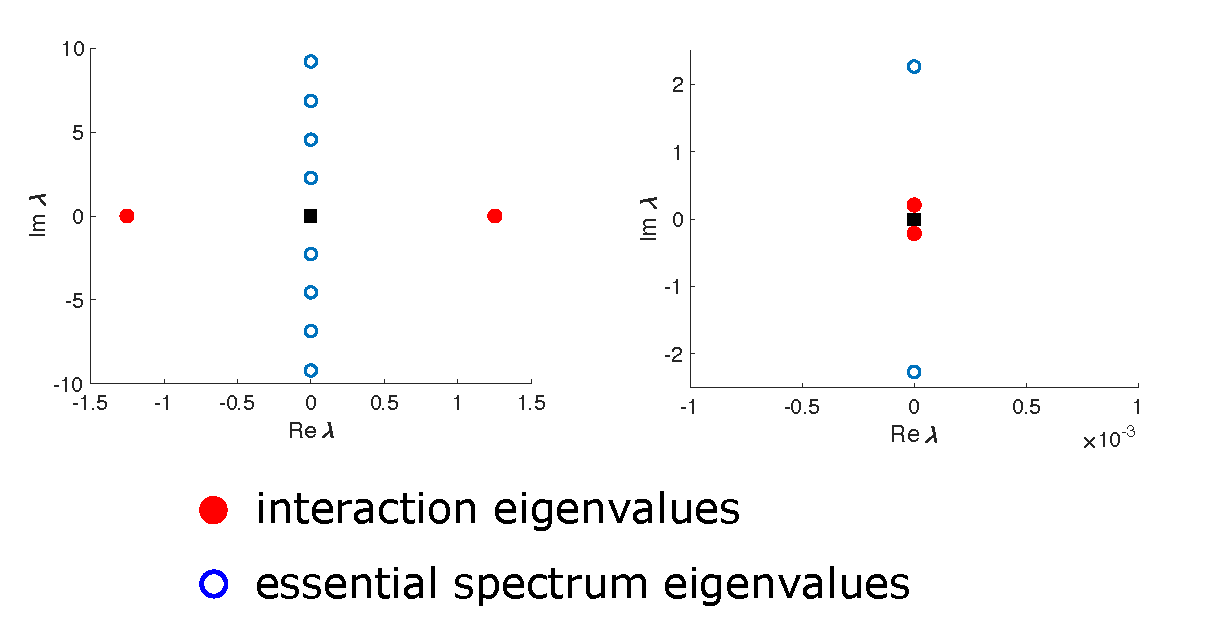
\includegraphics[width=12cm]{images/numericspec.eps}
		\end{center}
		\end{figure}
\end{frame}

\begin{frame}
\frametitle{Eigenvalue pattern determined by geometry} 
    \begin{block}{Theorem [P.]}
    For a periodic 2-pulse, as long as the period $X = X_0 + X_1$ is not ``too large'', we have the following interaction eigenvalue pattern
    	\begin{figure}
		\begin{center}
		\includegraphics[width=7cm]{images/2pitchforkcoloreig.eps}
		\end{center}
		\end{figure}
    \end{block}
\end{frame}

\begin{frame}
	\frametitle{Eigenvalue collision}
	\large
	What happens as the period $X$ increases?
	\begin{itemize}
		\item Interaction eigenvalues are (roughly) constant
		\vspace{0.5cm}
		\item Essential spectrum eigenvalues move towards the origin
		\vspace{0.5cm}
		\item Essential spectrum eigenvalue (positive Krein signature) will collide with interaction eigenvalue (negative Krein signature)
		\vspace{0.5cm}
		\item Generically, this will cause a pair of eigenvalues to move off of the imaginary axis
	\end{itemize}
\end{frame}

\begin{frame}
	\frametitle{Eigenvalue collision}
	As period $X$ increases...
	\begin{center}
		\includemedia[
		     width=8cm,height=6cm,
		     activate=pageopen,
		     addresource=videos/Kreincollision.mp4,
		     flashvars={
		         source=videos/Kreincollision.mp4
		        &autoPlay=false
		     }
		]{}{VPlayer.swf} 
	\end{center}
\end{frame}


\begin{frame}
	\frametitle{Krein bubbles}
		\begin{figure}
		\begin{center}
		\includegraphics[width=12cm]{images/KreinBubbleTop.eps} \\
	\includegraphics[width=12cm]{images/KreinBubbleBottom.eps}
		\end{center}
		\end{figure}
		\begin{center}
		Cartoon of Krein bubble
		\end{center}
\end{frame}

\begin{frame}
	\frametitle{Krein bubbles}
		\begin{figure}
		\begin{center}
		\includegraphics[width=8cm]{images/Kreinbubble1.eps}
		\end{center}
		\end{figure}
		\begin{center}
		Real and imaginary parts of eigenvalues near Krein bubble \\
		(Parameter continuation with AUTO)
		\end{center}
\end{frame}

\begin{frame}
	\frametitle{Krein bubbles}
	\begin{block}{Theorem [P.]}

		\begin{itemize}
		\item Krein bubbles occur when an essential spectrum eigenvalue collides with an interaction eigenvalue on the imaginary axis.

		\item Radius of $m$-th Krein bubble in the complex plane is $\sqrt{\dfrac{R}{m}}$
		\begin{align*}
		R = \frac{M_c^2 }{2 \pi M^2 c } |\lambda_*|^5 X_0^2 + \text{``h.o.t.''}
		\end{align*}
		\begin{itemize}
			\item $\lambda_*$ is the interaction eigenvalue
			\item $X_0$ is the distance between the two peaks
			\item $c$ is the wavespeed
			\item $M$ and $M_c$ are Melnikov-type integrals
		\end{itemize}
		\end{itemize}
	\end{block}
\end{frame}

\begin{frame}
	\frametitle{Subsequent Krein bubbles}
	First five Krein bubbles
		\begin{figure}
		\begin{center}
		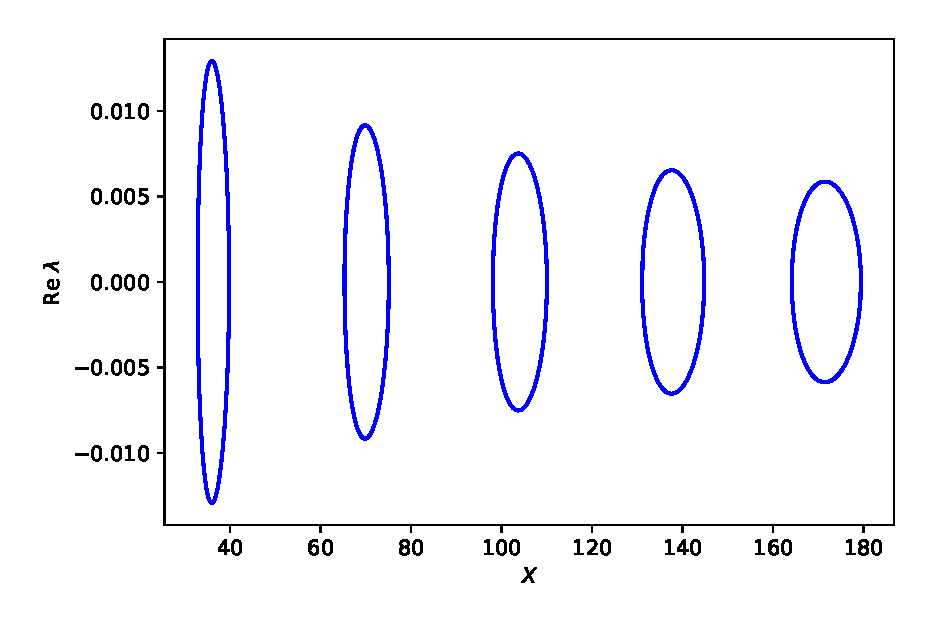
\includegraphics[width=8cm]{images/5bubbles.eps}
		\end{center}
		\end{figure}
	\begin{itemize}
		\item Krein bubbles approximately evenly spaced in $X$
		\item Subsequent Krein bubbles get wider in $X$
		\item Size of $m$-th Krein bubble in $X$ scales as $\sqrt{m}$
	\end{itemize}
\end{frame}

\begin{frame}
	\frametitle{Krein bubbles can collide}
	After a critical value of $X$ is reached
		\begin{figure}
		\begin{center}
		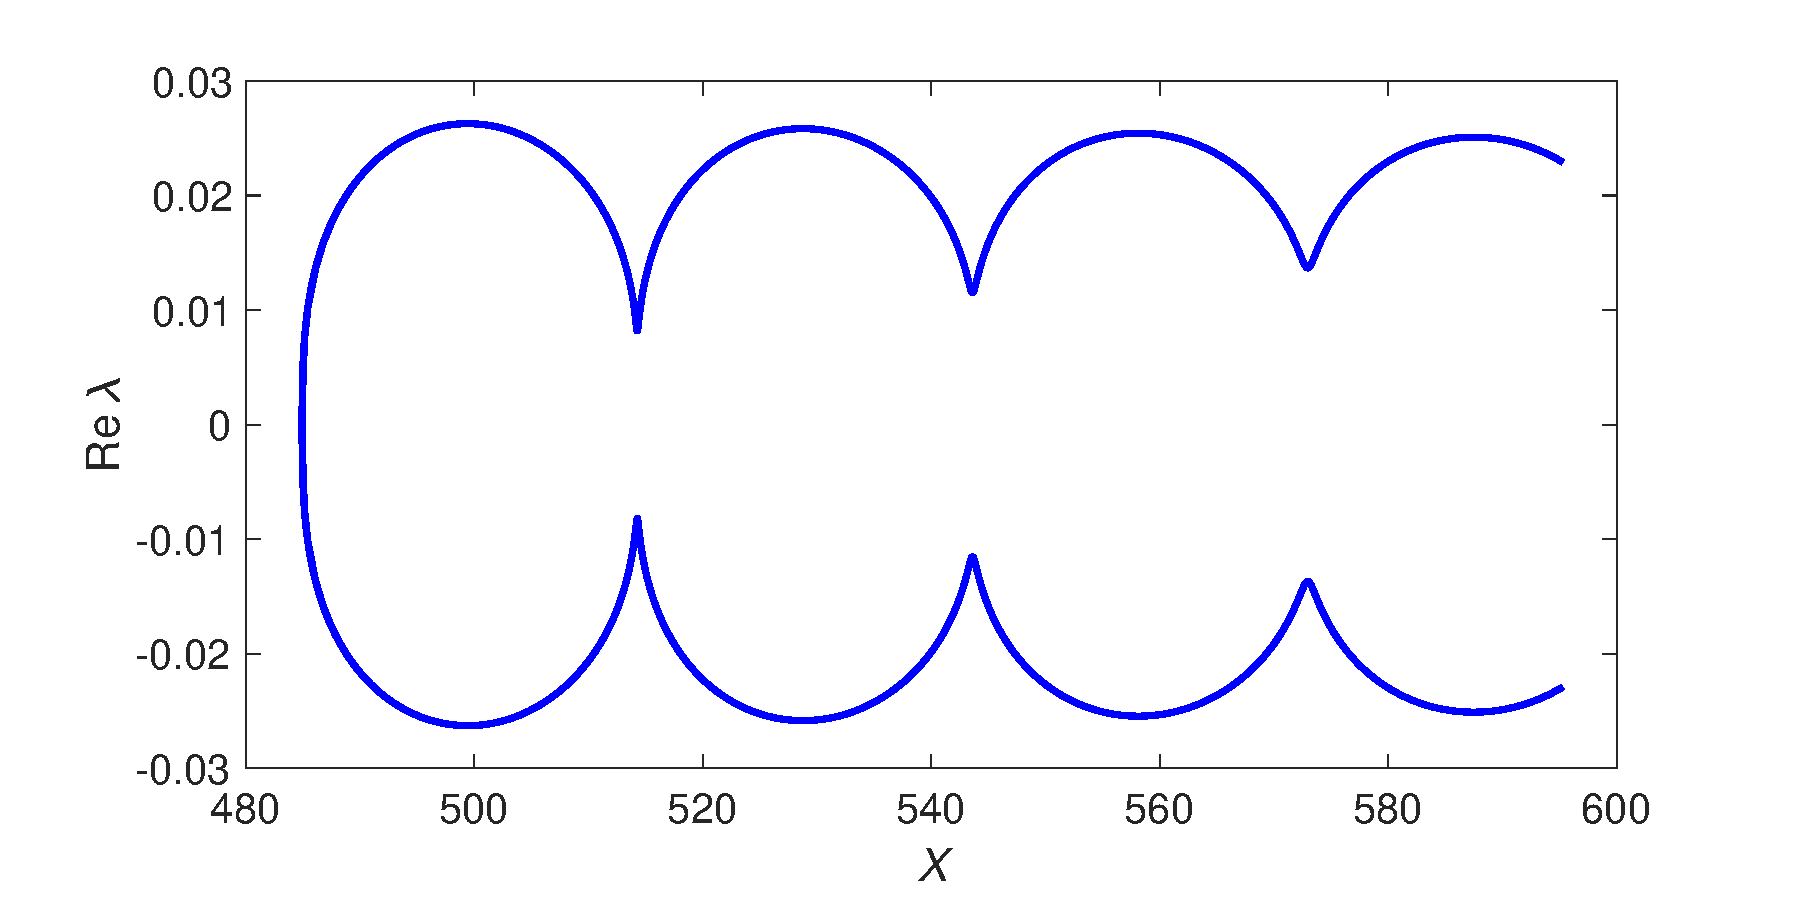
\includegraphics[width=8cm]{images/KreinBubbleCollision.eps}
		\end{center}
		\end{figure}
	\begin{itemize}
		\item Neighboring Krein bubbles overlap
		\item Always an eigenvalue with positive real part
		\item All periodic double pulses are unstable for sufficiently large $X$
	\end{itemize}
\end{frame}

\begin{frame}
	\frametitle{Conclusions and future directions}
	\begin{itemize}
		\item Spectrum of periodic multi-pulses depends on their geometry
		\vspace{0.5cm}
		\item Instability bubbles occurs when eigenvalues collide on the imaginary axis
		\vspace{0.5cm}
		\item Future directions
		\begin{itemize}
		\item Use time-stepping to see how perturbed multi-pulses evolve
		\item What is nature of instability represented by Krein bubble in periodic case?
		\item Investigate similar phenomena in other systems, e.g. dark solitons in discrete NLS
		\end{itemize}
	\end{itemize}
\end{frame}


\begin{frame}
	\frametitle{References}
	\fontsize{12}{7.2}\selectfont
	\begin{enumerate}
		\item Parker R. and Sandstede B. \emph{Periodic multi-pulses and spectral stability in Hamiltonian PDEs with symmetry}. arXiv:2010.05728.
		\item Buffoni B. and S\'er\'e E. \emph{A global condition for quasi-random behaviour in a class of conservative systems}. Commun. Pure Appl. Math., 49 (1996), 285-305.
		\item Chugunova M and Pelinovsky P. \emph{Two-pulse solutions in the fifth-order KdV equation: Rigorous theory and numerical approximations}. Discrete and Continuous Dynamical Systems, Series B 8.4 (2007), 773-800.
		\item Groves M D. \emph{Solitary-wave solutions to a class of fifth-order model equations}. Nonlinearity, 11 (1998), 341-353.
		\item Sandstede B. \emph{Stability of multiple-pulse solutions}. Trans. Am. Math. Soc., 350 (1998), 429-472.
	\end{enumerate}
\end{frame}

\begin{frame}
	\fontsize{16}{7.2}\selectfont
\begin{center}
		Questions?

		\begin{figure}[H]
		\begin{tabular}{c}
		\includegraphics[width=0.65\linewidth]{images/babyelephant4.jpg} 
		\end{tabular}
		\end{figure}

	\end{center}
\end{frame}

\begin{frame}
	\frametitle{Time stepping}
	\fontsize{14}{7.2}\selectfont
	\begin{itemize}
		\item What might this imply for the PDE?
		\item How do perturbations evolve in time?
		\item Suppose 2-pulse eigenvalue pattern is
		\begin{figure}
		\begin{center}
		\includegraphics[width=5cm]{images/DPeigpattern.eps}
		\end{center}
		\end{figure}
		\item We are ignoring the essential spectrum
		\item What does this imply for PDE dynamics?
	\end{itemize}
\end{frame}

\begin{frame}
	\frametitle{Time stepping}
	\fontsize{14}{7.2}\selectfont
	\begin{itemize}
		\item What happens near the 2-pulse equilibria?
		\vspace{0.5cm}
		\item Time-stepping scheme:
		\begin{itemize}
			\item Chebyshev polynomial spectral discretization in space
			\item Dirichlet/Neumann boundary conditions
			\item Crank-Nicolson/Adams-Bashforth 2 IMEX scheme for time-stepping
		\end{itemize}
		\vspace{0.5cm}
		\item Initial condition: ``pull apart'' 2-pulses and let go!
	\end{itemize}
\end{frame}

\begin{frame}
	\frametitle{Timestepping results}
	\fontsize{14}{7.2}\selectfont
	\begin{figure}[H]
	\begin{center}
	\begin{tabular}{cc}
	\includegraphics[width=0.4\linewidth]{images/waterfallunstable.eps} &
	\includegraphics[width=0.4\linewidth]{images/waterfallstable.eps} \\
	Unstable double pulse & Neutrally stable double pulse \\
	Repels & Oscillates
	\end{tabular}
	\end{center}
	\end{figure}
\end{frame}
 
\end{document}